\section{JSON}

JSON ou Javascript Object Notation é um formato de serialização de dados human-readable baseado em texto com especificação padronizada e parcialmente descritivo. Foi desenvolvido por Douglas Crockford com o objetivo de representar dados em uma maneira simples, leve e flexível através da redução na sobrecarga de marcações comparado ao formato XML.

Por ter se adaptado bem no ambiente de aplicações distribuídas, este formato acabou sendo amplamento utilizado por empresas como principal forma de represetação de dados serializados em seus serviços. A figura 2 mostra claramente a preferência do formato JSON por desenvolvedores ao criar novas APIs. \cite{Duvander2013}

\begin{figure}[h]
  \centering
  \resizebox{\columnwidth}{!}{
    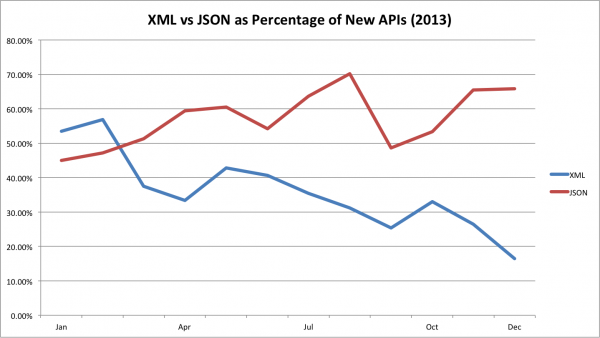
\includegraphics[width=\textwidth,height=\textheight,keepaspectratio]{figuras/xml-vs-json.png}
  }
  \caption{Porcentagem de novas APIs em XML e JSON}
\end{figure}

Na sua essência, JSON foi construído com base em 4 tipos primitivos de dados e outros 2 para composição. Cada tipo possui seu respectivo correspondente na maioria das linguagens de programação, embora possam ser identificados por nomes diferentes. \cite{Droettboom2015}

\begin{table}[ht!]
  \centering
  \resizebox{\columnwidth}{!}{
    \begin{tabular}{|c|c|c|c|c|}
      \hline
      Tipo & Exemplo de Valor \\
      \hline
      Object & \mintinline{c}{ {"key1": "value1", "key2": "value2"} } \\
      Array & \mintinline{c}{ ["first", "second", "third"] } \\
      Number & \mintinline{c}{ 1, -1, 2.9999 } \\
      String & \mintinline{c}{ "This is a string" } \\
      Boolean & \mintinline{c}{ true, false } \\
      Null & \mintinline{c}{ null } \\
      \hline
    \end{tabular}
  }
  \caption{Exemplo de tipos de valores em JSON}
\end{table}

Através da composição de listas, objetos e tipos primitivos, é possível representar complexas estruturas de dados que aplicações possam vir a serializar. No entanto, não existe um único padrão de representação em JSON, uma vez que dado uma estrutura para serializar, é possível representá-lo de inúmeras maneiras. \cite{Droettboom2015}

Por exemplo, a seguir estão duas formas diferentes de representação em JSON para os mesmo dados de uma entidade “pessoa”:

\begin{figure}[h]
  \centering
  \inputminted[frame=single,framesep=10pt]{javascript}{anexos/pessoa.json}
  \caption{Primeiro exemplo de representação JSON}
\end{figure}

\begin{figure}[h]
  \centering
  \inputminted[frame=single,framesep=10pt]{javascript}{anexos/pessoa-2.json}
  \caption{Segundo exemplo de representação JSON}
\end{figure}

Ambas representações são válidas, apesar da figura 4 estar representando dados em uma estrutura mais formal que a outra. No entanto, por ser um formato não descritivo, a responsabilidade de entender o que está sendo representado em JSON vai depender da análise crítica ou conhecimento prévio dos desenvolvedores. Já uma máquina, sem conhecer o contexto, não saberia como interpretar os dados de forma correta. \cite{Droettboom2015}

Para isso, será abordado em seguida um dos formatos de descrição existentes hoje para descrever estruturas JSON utilizados no projeto.

\subsection[JSON Schema]{JSON Schema}

JSON Schema é uma linguagem de definição projetada para descrever estruturas de dados JSON por meio de esquemas. Foi proposta em 2009 por Kris Zyp com objetivo de fornecer um contrato para que aplicações soubessem como trabalhar e interagir com estruturas de dados. Por meio deste, é possível prever representações e assim realizar operações de validação, documentação, navegação hyperlink e controle de iteração.

Por ser uma linguagem de simples uso, para modelar um esquema basta construir um objeto JSON utilizando um subconjunto válido de chaves especias descritas pela linguagem. No entanto, funcionalidades como descrição de estruturas multimídia\footnote{
  Imagens, videos, audio digital.
} e a navegação de dados são apenas disponibilizadas no formato JSON Hyper-Schema, uma variação da linguagem de especificação. \cite{Jackson2016}

\begin{figure}[H]
  \centering
  \begin{minted}[frame=single,fontsize=\small]{javascript}
    {
      "\$schema": "http://json-schema.org/draft-04/schema#",
      "title": "Pessoa",
      "description": "Uma pessoa",
      "type": "object",
      "required": ["nome", "aniversario"],
      "properties": {
        "nome": {
          "type": "string"
        },
        "aniversario": {
          "type": "string"
        },
        "cidade": {
          "type": "string"
        }
      }
    }
  \end{minted}
  \caption{JSON Schema para Figura 3}
\end{figure}

\begin{figure}[H]
  \centering
  \begin{minted}[frame=single,fontsize=\small]{javascript}
    {
      "\$schema": "http://json-schema.org/draft-04/hyper-schema#",
      ...
      "properties": {
        ...
        "foto": {
          "media": {
            "binaryEncoding": "base64",
            "type": "image/png"
          }
        }
      },
      "links": [
        {
          "rel": "foto",
          "href": "/{id}.png",
          "mediaType": "image/png"
        }
      ]
    }
  \end{minted}
  \caption{JSON Hyper-Schema para Figura 3}
\end{figure}

Ao exemplo das figuras 5 e 6, ambos os esquemas asseguram que, dado uma estrutura JSON, para que esta seja reconhecida como uma entidade “pessoa” deve conter as propriedades "nome" e "aniversario" com valores do tipo "string". Já na figura 6, além das estruturas definidas pela figura 5, é descrito uma nova propriedade "foto" do tipo multimídia, além de como navegar em busca desta informação.

Em casos onde a complexidade de um esquema começa a crescer, é comum a definição de sub-esquemas através da chave “definitions”. Desta forma, podem ser referenciadas pela chave "\$ref" permitindo o reuso de estruturas dentro de um esquema. Vale lembrar que a chave “definitions” é apenas um mecanismo útil para definir esquemas em um lugar comum, entretanto, não sugerem que estas propriedades sejam validadas em um objeto ao menos que referenciadas em outras estruturas do esquema. \cite{Leach2014}

\begin{figure}[H]
  \centering
  \begin{minted}[frame=single,fontsize=\small]{javascript}
    {
      "\$schema": "http://json-schema.org/draft-04/hyper-schema#",
      ...
      "definitions": {
        "cidade": {
          "type": "string",
          "properties": {
            "nome": { "type": "string" },
            "estado": { "type": "string" },
            "pais": { "type": "string" }
          }
        }
      },
      "properties": {
        ...
        "cidade": {
          "\$ref": "#/definitions/cidade"
        }
      },
      "links": [
        ...
        {
          "rel": "cidade",
          "href": "/{id}/cidade",
          "targetSchema": {
            "\$ref": "#/definitions/cidade"
          }
        }
      ]
    }
  \end{minted}
  \caption{JSON Hyper-Schema para Figura 4 usando \$ref}
\end{figure}

Como boa prática, é recomendado (mas não necessário) o uso da chave especial “\$schema” para determinar quando uma estrutura JSON está sendo representada em forma de esquema. Na tabela 3, é descrito algumas das chaves especiais usadas para descrever objetos em esquemas. \cite{Droettboom2015}

\begin{table}[ht!]
  \centering
  \begin{tabular}{|c|c|}
    \hline
    Chave & Descrição \\
    \hline
    \$schema & Identificador de versão \\
    \hline
    type & Tipo de dado \\
    \hline
    title & Nome da estrutura \\
    \hline
    description & Propósito da estrutura \\
    \hline
    required & Lista de propriedades com presença obrigatória \\
    \hline
    properties & Propriedades usadas para validar uma estrutura \\
    \hline
    definitions & Propriedades (sub-esquemas) para referência \\
    \hline
    ... & ... \\
    \hline
    links & Lista de Link Description Objects (LDO) \\
    \hline
  \end{tabular}
  \caption{Subconjunto de chaves especiais JSON Schema}
\end{table}

De certa forma, JSON Schema continua sendo uma das únicas tentativas sérias de propor uma linguagem de definição para o formato. Contudo, ainda está longe de ser considerada padrão, mas já há um número crescente de aplicações que suportam o formato, além de uma quantidade significativa de ferramentas que permitem sua validação. \cite{PezoaEtAl2016}

Vale lembrar também que, segundo Leach, com o recente surgimento de grandes formatos de descrição de APIs ao longo dos últimos anos, JSON Schema tem-se tornado uma ótima opção para descrever, não apenas estruturas de requisição e resposta JSON mas também como documentar e navegar pontos de acesso em API's. \cite{Leach2014}

No próximo capítulo será feito uma abordagem sobre um dos estilos de arquitetura mais utilizados hoje em dia em APIs web, além de soluções encontradas no mercado para descrição destes serviços.

